\chapter{GW in the post-inflationary universe}
In this section we will explore the evolution of gravitational waves in the post-inlationary universe: understanding this is fundamental to predict how the primordial power spectrum we found can impact present observable and which phenomena can magnify or reduce the resulting signal. To begin with we will describe free propagation of gravitational waves in the different eras of the universe to then introduce interactions that can alter this.

\section{Free gravitational waves in FRW universe}
While dealing with gravitational waves in inflationary scenario, we already gave the action of gravitational waves on the FRW background
\begin{equation*}
    \mathcal{S} [h_{ij}]=\frac{1}{64\pi G}\int d^4xa^2\Big[(h'_{ij})^2-(h_{ij,k})^2\Big]=\frac{1}{64\pi G}\sum_{\lambda=+,\times}\int d^4xa^2\Big[(h'_{(\lambda)})^2-(h_{(\lambda),k})^2\Big],
\end{equation*}
where we used the decomposition of gravitational waves in their two polarizations
$$h_{ij}=\sum_{\lambda=+,\times}h_{(\lambda)}\boldsymbol\epsilon^\lambda_{ij},\qquad \text{with }\boldsymbol{\epsilon}^\lambda_{ij}\boldsymbol{\epsilon}^{(\lambda) ij}=1.$$
Varying this action the equation of motion for both polarizations reads
\begin{equation}
    h''+2\frac{a'}{a}h'-\boldsymbol{\nabla}^2h=0,\label{eq:EOM_GW_FREE}
\end{equation} 
where we suppressed the label $\lambda$ since the dynamics is identical for both polarizations. To solve the above we shall choose a background on which the gravitational wave propagates: we will consider \emph{radiation dominated} and \emph{matter dominated}  backgrounds. In general, the Friedmann equation gives $a(\tau)\propto\tau^{2/(3\omega+1)}$, which results in two different equations of motion: in Fourier space they read
\begin{align}
    \tilde h_k''+2\frac{\beta}{\tau}\tilde h_k'+\boldsymbol{k}^2\tilde h_k=0,\qquad \beta=\begin{cases}
        1\ \text{radiation dominated,}\\
        2\ \text{matter dominated.}
    \end{cases}\label{eq:GW_Fourier}
\end{align}
We recognize that the above equation can be turned in the Bessel equation by defining the variable $x\defeq k\tau$ and matching $J_\nu=x^\alpha\tilde h_k$
\begin{align*}
    0&=\frac{d^2\tilde h_k}{dx^2}+2\frac{\beta}{x}\frac{d\tilde h_k}{dx}+\tilde h_k=\frac{d^2}{dx^2}J_\nu x^\alpha+2\frac{\beta}{x}\frac{d}{dx}J_\nu x^\alpha+J_\nu x^\alpha\\ &=x^\alpha\bigg[\frac{d^2J_\nu}{dx^2}+\frac{2\alpha}{x}\frac{dJ_\nu}{dx}+\alpha\frac{\alpha-1}{x^2}J_\nu+2\frac{\beta}{x}\bigg(\frac{dJ_\nu}{dx}+\frac{\alpha}{x}J_\nu\bigg)+J_\nu\bigg]\\
    &=x^\alpha\bigg[\frac{d^2J_\nu}{dx^2}+2\frac{\alpha+\beta}{x}\frac{dJ_\nu}{dx}+\bigg(1+\alpha\frac{\alpha-1}{x^2}+\frac{2\alpha\beta}{x^2}\bigg)J_\nu\bigg]
\end{align*}
then by fixing $\alpha$ such that $\alpha+\beta=1/2$ 
$$\frac{d^2J_\nu}{dx^2}+\frac{1}{x}\frac{dJ_\nu}{dx}+\bigg(1+\frac{(\beta-\frac{1}{2})^2}{x^2}\bigg)J_\nu=\frac{d^2J_\nu}{dx^2}+\frac{1}{x}\frac{dJ_\nu}{dx}+\bigg(1-\frac{\nu^2}{x^2}\bigg)J_\nu=0.$$
The above shows that the solutions to the gravitational wave equation are the Bessel function, of order $\nu=\beta-\tfrac12$ times $(k\tau)^{-\beta+1/2}$,
$$\tilde h_k(\tau)=(k\tau)^{\frac{1}{2}-\beta}\bigg[C_1(\mathbf{k}) J_{\beta-\frac{1}{2}}(k\tau)+C_2(\mathbf{k}) Y_{\beta-\frac{1}{2}}(k\tau)\bigg],$$
where $J_\nu$ and $Y_\nu$ are the \emph{Bessel functions of the first and second kind}, respectively, and $\beta$ depends on the background cosmology. Note that the above solution can be expressed in a nicer form by using that the \emph{spherical Bessel functions} can be expressed as $j_\ell(x)=\sqrt{\frac{\pi}{2x}}J_{\ell+\frac{1}{2}},\ y_\ell(x)=\sqrt{\frac{\pi}{2x}}Y_{\ell+\frac{1}{2}}$, by reabsorbing extra factors and $k^{\beta}$ in the two constants $C_1$ and $C_2$ and recalling that $a\propto\tau^{\beta}$, so that we have
\begin{equation}
    \label{eq:free_GW_sol}
    \tilde h_k(\tau)=C_1(\mathbf{k})\tau\frac{j_{\beta-1}(k\tau)}{a(\tau)}+C_2(\mathbf{k})\tau\frac{y_{\beta-1}(k\tau)}{a(\tau)}.
\end{equation}
Note that the above solution holds also during slow-roll inflation, when a simple calculation gives $\beta\approx-1$. Lastly, let us appreciate that super Hubble horizon and sub Hubble horizon regimes we recover the behaviors which we already discovered studying inflation: from equation \eqref{eq:EOM_GW_FREE}, in the limit $k^2\gg a'/a=a H$ oscillating modes are displayed at sub Hubble horizon scales while for $k^2\ll\ a'/a=a H$ the solution reads:
$$\tilde h_k(\tau)=C_1(\mathbf k)+C_2(\mathbf k)\int\frac{d\tau}{a^2},$$ which is a combination of a constant mode and a mode that decays as the universe expands.
\section{Interacting GW}
\subsection{Neutrino damping}
\label{sec:neutrino_damping}
The previous section was devoted to study the evolution of tensor perturbations, namely primordial gravitational waves, in the free case, when no matter perturbation is coupled to these modes. Weinberg \cite{Weinberg_nu_dump} showed that free streaming neutrinos (neutrinos that decoupled from the plasma and can move freely without scatterings) can source anisotropic stress that then couples with the gravitational waves reducing their amplitudes after having crossed back the horizon. In this section we will illustrate this behavior.

Perturbing the Einstein field equations with tensor perturbations, in general results in the following
$$\delta G_{\mu\nu}=8\pi G\delta T_{\mu\nu}\quad \Rightarrow\qquad h''_{ij}+2\frac{a'}{a}h'_{ij}-\boldsymbol{\nabla}^2 h_{ij}=16\pi G a^2\delta T_{ij},$$
where $h_{ij}$ is the usual transverse traceless tensor characteristic of gravitational waves. When we studied matter perturbations (section \ref{sec:perturbations}) we allowed the stress-energy tensor to contain a spatial transverse traceless contribution called \emph{anisotropic stress}. From the above equation it is clear that, accordingly to the symmetries of $h_{ij}$, the only term that can appears at the right-hand side, from the stress-energy tensor, is the anisotropic stress:
\begin{equation}
    h''_{ij}+2\frac{a'}{a}h'_{ij}-\boldsymbol{\nabla}^2 h_{ij}=16\pi G a^2\pi_{ij}.\label{eq:GW_EOM_stress}
\end{equation}
We will now proceed to show that a non-zero $\pi_{ij}$ can be sourced by free streaming neutrinos, nevertheless keep in mind that an anisotropic stress can be sourced also by other phenomena as magnetic fields or photons.

We now need to understand the behavior of neutrinos in the early universe: this is described by the \emph{Boltzmann equation}. Essentially, the Boltzmann equation describes the time evolution of the \emph{phase space distribution} $f(x,\mathbf p)$ of a determined specie, in general it reads
\begin{equation}
    \hat{L}[f]=C[f],\quad \text{with } \hat{L}[f]\defeq\frac{df}{dt}.
\end{equation}
The left hand-side is the \emph{Liouville operator}, which describes the evolution of $f(x,\mathbf p)$ accounting for the effects of curved spacetime, while the right hand-side is the \emph{collision operator}, which instead describes all the possible interactions among the species in the plasma. Since we will consider decoupled neutrinos the collision term will be set to zero from now on, hence the Boltzmann equation will be just a conservation equation. By the chain rule, the Liouville operator can be expressed in its explicit form
\begin{align*}
    \hat L[f]&=\frac{df}{dt}= \frac{\partial f}{\partial t}+\frac{\partial f}{\partial x^i}\frac{dx^i}{dt}+\frac{\partial f}{\partial p_i}\frac{dp_i}{dt},
\end{align*}
where we can evaluate all the remaining total derivatives with respect to time from the relativistic equations of motion:
$$\frac{dx^i}{dt}=\frac{dx^i/d\lambda}{dx^0/d\lambda}=\frac{p^i}{p^0},\qquad \frac{dp^i}{d\lambda}=\frac{dp^i}{dt}p^0=-\Gamma^i_{\mu\nu} p^\mu p^\nu,$$
however note that in the Lioville operator we chose to use $p_i$ as the momentum variable of the phase space, a simple calculation yields
\begin{align*}
        \frac{dp_i}{dt}=&\frac{d}{dt}g_{ij}p^j=g_{ij,0}p^j+h_{ij,k}p^ip^k+g_{ij}\frac{dp^j}{dt}\\
        &=g_{ij,0}p^j+g_{ij,k}p^jp^k-\Gamma^{i}_{\mu\nu}\frac{p^\mu p^\nu}{p^0}\\
        &=g_{ij,0}p^j+g_{ij,k}p^jp^k-2\frac{1}{2}g^{ik}g_{jk,0}p^j-\frac{1}{2}g^{ih}(g_{hk,j}+g_{hj,k}-g_{jk,h})\frac{p^kp^j}{p^0}\\
        &=\frac{1}{2}g_{jk,i}\frac{p^kp^j}{p^0}
\end{align*}
In this way the Boltzmann equation reads
\begin{equation}
    \frac{\partial f}{\partial t}+\frac{\partial f}{\partial x^i}\frac{p^i}{p^0}+\frac{\partial f}{\partial p_i}\frac{p^jp^k}{2p^0}g_{jk,i}=0. \label{eq:Boltzmann_neutrinos}
\end{equation}
We will now assume that initially at some time $t_1$, just after decoupling from the plasma, neutrinos are described by a \emph{Fermi-Dirac} distribution with zero chemical potential:
$$f(\mathbf{x},\mathbf{p},t_1)\defeq\bar f(\mathbf{x},\mathbf{p})=\bigg[\exp\bigg(\sqrt{g^{ij}(\mathbf x,t_1)p_ip_j}/k_B T_1\bigg)+1\bigg]^{-1},$$
where $T_1$ is the temperature of the plasma at $t_1$ and $k_B$ is the Boltzmann constant. In the absence of perturbations the Boltzmann equation would maintain the above solution as time evolves. However, introducing metric perturbations we now have to allow for perturbations $\delta f$ of the phase space distribution to arise with the condition $\delta f(\mathbf x,\mathbf p, t_1)=0$, so that overall we find
$$f(x,\mathbf p)=\bigg[\exp\bigg(\sqrt{g^{ij}(\mathbf x,t_1)p_ip_j}/k_B T_1\bigg)+1\bigg]^{-1}+\delta f(\mathbf{x},\mathbf{p},t).$$
By plugging the above in the Boltzmann equation \eqref{eq:Boltzmann_neutrinos} and keeping only up to first order terms, the equation of motion for the perturbations $\delta f$ is obtained:
\begin{align*}
   0&=\frac{\partial \delta f}{\partial t}+\frac{\partial \delta f}{\partial x^i}\frac{p^i}{p^0}+\frac{p^i}{p^0}\frac{\partial }{\partial x^i}\frac{1}{e^{\sqrt{p_ip^j}/k_BT_1}+1}+\frac{p^jp^k}{2p^0}g_{jk,i}\frac{\partial }{\partial p_i}\frac{1}{e^{\sqrt{p_ip^j}/k_BT_1}+1}\\&= \frac{\partial \delta f}{\partial t}+\frac{\partial \delta f}{\partial x^i}\frac{\hat p^i}{a}+\frac{\hat p^k}{a}\bar f'(p)\frac{p_ip_j}{2p^0}\tensor{g}{^i^j_,_k}(\mathbf{x},t_1)+\bar f'(p)p^i\frac{p^jp^k}{2p^0}g_{jk,i}(\mathbf x, t) \\&= \frac{\partial \delta f}{\partial t}+\frac{\partial \delta f}{\partial x^i}\frac{\hat p^i}{a}-\frac{p}{2a}\bar f'(p)\hat p_k\hat p_i\hat p_j\tensor{h}{_i_j_,_k}(\mathbf{x},t_1)+\frac{p}{2a}\bar f'(p)p_k\hat p_j\hat p_ih_{ji,k}(\mathbf x, t)\\
   &\Longrightarrow\qquad \frac{\partial \delta f}{\partial t}+\frac{\partial \delta f}{\partial x^i}\frac{\hat p^i}{a}=\frac{p}{2a}\bar f'(p)\hat p_k\hat p_i\hat p_j[\tensor{h}{_i_j}(\mathbf{x},t_1)-h_{ij}(\mathbf x, t)]_{,k},
\end{align*}
where the prime indicates derivatives with respect to the argument of the function and $\hat p^i\defeq p^i/p$ with $p\defeq{\sqrt{p_ip_j\delta^{ij}}}$. This differential equation can be integrated quite easily if we assume that the $\mathbf x$ dependence of $h_{ij}$ and $\delta f$ is solely due to a factor $e^{i\mathbf{k\cdot x}}$ and by defining a new variable $u= k\int_{t_1}^{t}dt'/a(t')$: in this way we have
$$\frac{a}{k}\frac{\partial \delta f}{\partial t}+i\delta f \mathbf{\hat p\cdot\hat k}=\frac{\partial}{\partial u}\bigg(\delta f e^{i\mathbf{\hat p\cdot\hat k}u}\bigg)=i\frac{p}{2}\bar f'(p)\mathbf{\hat p\cdot\hat k}\hat p_i\hat p_j[\tensor{h}{_i_j}(t_1)-h_{ij}( t)]$$
which upon integration, with the initial condition $\delta f(t=t_1)=0$, gives
\begin{equation}
    \delta f(u,\mathbf p) = \frac{i}{2}\bar f'(p)\mathbf{\hat p\cdot\hat k}\hat p_i\hat p_j\int_{0}^{u}du'e^{i\mathbf{\hat p\cdot\hat k}(u'-u)}(\tensor{h}{_i_j}(0)-h_{ij}(u')).
\end{equation}
We now proceed to compute the anisotropic stress tensor $\pi_{ij}$, which accordingly to our definition in section \ref{sec:perturbations} corresponds to the transverse traceless spatial part of the stress-energy tensor, that for a given phase space distribution reads
\begin{align*}
    \tensor{T}{^i_j}=\frac{1}{\sqrt{\det g}}\int dp_1dp_2dp_3\ f(\mathbf x,\mathbf p,t)\frac{p^ip_j}{p^0}.
\end{align*}
In the above equation three first order terms are produced: by the perturbation $\delta f$ and by the momenta $p^i$ and $p^0$ through the metric ($p^i=g^{ij}p_j$ and $p^0=\sqrt{g^ijp_ip_j}$). Combining these contributions together Weinberg shows that the anisotropic stress reads
\begin{equation}
    \pi_{ij}=-4\bar\rho_\nu(u)\int_0^u dU\ K(u-U)h'_{ij}(U),\quad \text{where}\quad K(s)\defeq\frac{1}{16}\int_{-1}^{+1}dx(1-x^2)^2e^{ixs},\label{eq:pi_ij_neutrinos}
\end{equation}
and again the prime indicates derivatives with respect to the argument of the function while $\bar\rho_\nu$ is the background energy density of neutrinos. Lastly, solving the above kernel integral yields
\begin{equation*}
    K(s)=-\frac{\sin s}{s^3}-3\frac{\cos s}{s^4}+3\frac{\sin s}{s^5}.
\end{equation*}

The result \eqref{eq:pi_ij_neutrinos} can be plugged back in the equation of motion of gravitational waves \eqref{eq:GW_EOM_stress} to obtain an integro-differential equation for $h_{ij}$: 
\begin{align}
    h''_{ij}(u)+2\frac{a'}{a}h'_{ij}(u)+ h_{ij}(u)&=-\frac{64\pi G}{k^2} a^2\bar\rho_\nu(u)\int_0^u dU\ K(u-U)h'_{ij}(U)\nonumber\\
    &=-24f_\nu(u)\bigg(\frac{a'}{a}\bigg)^2\int_0^u dU\ K(u-U)h'_{ij}(U),\label{eq:GW_EOM_neutrinos}
\end{align}
where we assumed again $h_{ij}\propto e^{i\mathbf{k\cdot x}}$, then we changed the variable in equation \eqref{eq:GW_EOM_stress} to $u$ and in the second line we used the Friedmann equation to refactor the energy density of neutrinos into $f_\nu= \bar\rho_\nu/\bar\rho$. Lastly, as we have done in the previous sections we can decompose the tensor modes in their two polarizations, which both satisfy the above. 

Solutions for the equation we found can be approximated in the sub Hubble horizon limit during radiation domination ($a\propto\tau\propto u$), long after the decoupling of neutrinos so that $t_1\approx 0$. Considering three neutrino flavors, then $f_\nu$ takes the constant value of $0.40523$ and overall we get for each polarization
$$ h''(u)+\frac{2}{u}h'(u)+h(u)=-\frac{24f_\nu}{u^2}\int_{0}^{u}dU\ K(u-U)h'(U).$$
The factor $u^{-2}$, in the right-hand side, suppresses the effects of the anisotropic stress inside the Hubble horizon ($u=k\tau$) were the free solution \eqref{eq:EOM_GW_FREE} is recovered
$$h(u)\xrightarrow{u\to 0} \frac{A\sin(u+\delta)}{u},$$
with $A$ and $\delta$ are constants that must be computed numerically. Dicus and Repko \cite{Dicus_Repko} integrated equation \eqref{eq:GW_EOM_neutrinos} numerically expanding the solutions on the spherical Bessel functions $j_n(u)$,
\begin{equation}
    \label{eq:Tmodes_nu_damped}
    h(u)=\sum_{n\text{ even}}^{\infty}a_n j_n(u).
\end{equation}
 In their work they have computed the numerical coefficients $a_0=1,\ a_2=0.0243807,\ a_4=5.28424\times10^{-2},\ a_6= 6.13545\times10^{-3}.\ a_8=2.07534\times10^{-4},\ a_{10}=6.16273\times10^{-5},\ a_{12}=-4.78885\times10^{-6}$ and with smaller and smaller higher coefficients. 
 Moreover, considering that for $u\to0$ all the even order Bessel functions behave as $(-1)^{n/2}\sin(u)/u$, the factor $A$ can be approximated assume
$$A\approx \sum_{n=0}^{5}(-1)^n a_{2n}\approx 0.80313,$$
which shows that the effect of the anisotropic stress is to reduce the amplitude of horizon crossing tensor perturbations.

\subsection{Photon damping}
\label{sec:photon_damping}
A further interaction that can damp the amplitude of primordial gravitational waves is the interaction with photons. Without going in the details of the calculations, due to their symmetries, primordial gravitational waves are directly coupled to the quadrupole momentum of the photon anisotropies. This happens precisely because projecting the polarizations $\mathbf{e}_{ij}^\lambda$ onto the wave number vector yields\footnote{In the following calculation polarization basis introduced by Hu and White in \cite{HuWhite} has been used.}
$$\mathbf{e}_{ij}^{(\pm)}\hat k^i\hat k^j=\sin^2\theta[\cos^2\phi-\sin^2\phi\pm2i\sin\phi\cos\phi]=\sin^2\theta e^{\pm i2\phi}\propto Y_{2,\pm2}(\theta,\phi),$$
where $Y_{2,\pm2}(\theta,\phi)$ are the spherical harmonics of order $2$ and $m=\pm2$. Indeed, if we expand the phase space distribution, over an initial Planckian distribution, for small fluctuations in the temperature $\Theta(t,\mathbf x,\mathbf p)$ we obtain a perturbation proportional to $\Theta$ itself:
$$
f(t,\mathbf x,\mathbf p)=\bigg[\exp\bigg\{\frac{p}{k_B\bar T(1+\Theta)}\bigg\}-1\bigg]^{-1}\approx \frac{1}{e^{\frac{p}{k_b\bar T}}-1}-\Theta p\frac{\partial \bar f}{\partial p},
$$ 
where $\bar T$ is the average temperature and $\bar f$ is the Planckian distribution. This time, the anisotropic stress can be obtained by projecting the spatial components of the Fourier transformed stress-energy tensor onto the polarization $\mathbf{e}_{ij}^{\pm}$, which by the above result gives:
$$\tilde T^{ij}\mathbf{e}_{ij}^{\pm}\propto\mathbf{e}_{ij}^{(\pm)}\hat k^i\hat k^j\propto Y_{2,\pm2}(\theta,\phi).$$
Integrating over the solid angle of $\versor{k}$, the spherical harmonics will project the temperature anisotropies $\tilde\Theta$, giving at the end that the anisotropic stress associated to photons is encoded in the quadrupole momentum $\tilde \Theta_{2}^{(\pm2)}$. The precise result reads $\tilde\pi^{(\gamma)}=\tfrac85\tilde\Theta^{(2)}_2$ \cite{HuWhite}.
One can show that this quadrupole momenta is generated directly by primordial gravitational waves, hence creating a back reaction effect.

The equation of motion for the gravitational waves, in the presence of this anisotropic stress, reads in Fourier space
\begin{equation}
    \tilde h''_{ij}+2\frac{a'}{a}\tilde h'_{ij}+\boldsymbol{k}^2 \tilde h_{ij}=16\pi G a^2\tilde\pi^{(\gamma)}_{ij},\label{eq:GW_EOM_photons}
\end{equation}
where $\tilde\pi^{(\gamma)}_{ij}$ is the anisotropic stress sourced. This equation can be simplified by using the Friedmann equation in conformal time, $\mathcal{H}^2=\tfrac{8\pi G}{3}\bar\rho a^2$, and assuming radiation domination, $a\propto \tau$ and $\bar\rho=\bar\rho_\gamma+\bar\rho_\nu$. After having decomposed equation \eqref{eq:GW_EOM_photons} in the two polarizations, we can rewrite the anisotropic stress in terms of the photon anisotropy quadrupole momentum ($\tilde\pi^{(\gamma)}=\tfrac85\tilde\Theta^{(2)}_2$). Lastly, we assume the tight coupling limit, the limit in which photons scatterings are very frequent in the plasma and higher multipoles become negligible, so that $\tilde\Theta^{(2)}_2\approx-\tfrac43\tfrac{\tilde h'}{n_e\sigma_T a}$ \cite{HuWhite},
where $n_e$ is the electron number density and $\sigma_T$ is the Thomson cross-section. In this way we obtain 
$$
    \tilde h''_{k}+\frac{2}{\tau}\tilde h'_{k}+\boldsymbol{k}^2 \tilde h_{k}=-\mathcal{H}^2\frac{32(1-R\nu)}{15n_e\sigma_T a}\tilde h'_{k}\defeq -\Gamma_\gamma \tilde h'_k,
$$
where we defined $R_\nu\defeq\bar\rho_\nu/(\bar\rho_\gamma+\bar\rho_\nu)$. Note that since $a\times n_e\propto a^{-2}$, as well as $\mathcal{H}$ during radiation domination, overall $\Gamma_\gamma$ is constant. In the sub Hubble horizon limit we can neglect the term $\tfrac2\tau \tilde h'_k$ and the equation of motions turns into a damped harmonic oscillator. This means that in this regime the solution reads 
\begin{equation}
    \tilde h_k(\tau)\approx\tilde h_k^{\text{free}}(\tau)e^{-\frac{\Gamma_\gamma}{2}\tau},
\end{equation} 
which is the free solution damped of an exponential factor. On supehorizon scales the tensor modes are frozen and the damping can be neglected.
\subsection{Primordial magnetic fields}
In this section we will analyze a different interaction that can take place in the early universe and that can alter the evolution of gravitational waves enhancing their amplitude. Before the decoupling epoch the electric conductivity of the plasma was very high resulting in the total dissipation of any electric field present in the universe. Hence, in these extreme conditions, only stationary magnetic fields could survive and interact with the content of the universe. 

Consider the electromagnetic tensor 
$$F_{\mu\nu}= \nabla_\mu A_\nu - \nabla_\nu A_\mu=\partial_\mu A_\nu-\partial_\nu A_\mu=\begin{pmatrix}
    0 & -E_x & -E_y & -E_z \\
    E_x & 0 & B_z & -B_y \\
    E_y & -B_z & 0 & B_x \\
    E_z & B_y & -B_x & 0
\end{pmatrix},$$
where $A_\mu$ is the 4-potential while $E_i$ and $B_i$ are the electric and magnetic fields. The stress energy tensor of the electromagnetic field is given by 
$$
\tensor{T}{^\mu_\nu}=\frac{1}{4\pi}\bigg(F^{\mu\alpha}F_{\nu\alpha}-\frac{1}{4}\tensor{g}{^\mu_\nu} F^{\alpha\beta}F_{\alpha\beta}\bigg).
$$
For these a straight forward computation shows that, in the absence of electric fields, the stress-energy tensor reads
\begin{subequations}
    \begin{align}
    \tensor{T}{^0_0}=&\frac{1}{8\pi a^4}\bigg(B^2-\frac{1}{2}B^2\bigg)=\frac{1}{16\pi a^4}B^2,\label{eq:EM_Tensor_00}\\
    \tensor{T}{^0_i}=&0\label{eq:EM_Tensor_0i},\\
    \tensor{T}{^i_j}=&\frac{1}{8\pi a^4}\bigg(B^iB_j-\frac{1}{2}\tensor{\delta}{^i_j} B^2\bigg)=\frac{1}{8\pi a^4}\bigg(B^iB_j-\frac{1}{4}\tensor{\delta}{^i_j} B^2\bigg).\label{eq:EM_Tensor_ij}
\end{align}
\end{subequations}
We immediately recognize in the components \eqref{eq:EM_Tensor_ij} a pressure term plus a contribution that can result in an anisotropic stress: this shows that in the presence of primordial magnetic fields, tensor perturbations will be coupled to these. To explicitly obtain the anisotropic stress we can Fourier transform the magnetic field, then projecting $\tensor{\tilde T}{^i_j}$ with $P_{ij}=\delta_{ij}-\hat k_i\hat k_j$, to obtain just the transverse part, and lastly we remove its trace:
$$\tilde\pi_{ij}^{(B)}\defeq\tensor{\tilde T}{_h_k}(\tensor{P}{^h_i}\tensor{P}{^k_j}-\frac{1}{2}\tensor{P}{_i_j}\tensor{P}{^k^h}),$$
where the factor $\tfrac12$ corresponds to 2-dimensional space on which we project and $\hat{k}$ is the versor of the wave vector $\mathbf{k}$.\\
Since we know that Einstein filed equations couple gravitational waves to anisotropic stress, in Fourier space their equation of motion reads
\begin{equation}
     \tilde h''_{ij}+2\frac{a'}{a}\tilde h'_{ij}+\boldsymbol{k}^2 \tilde h_{ij}=16\pi G a^2\tilde\pi^{(B)}_{ij}.
\end{equation}
The peculiarity of this kind of source term is that, not being determined by the system of equations that describes all the cosmological perturbations, it is a generic forcing term that can magnify the amplitude of gravitational waves. 

In general, we model primordial magnetic fields as a stochastic background described by a 2- point function, in momentum space,
\begin{equation}
    \langle B_i(\mathbf{k})B^*_j(\mathbf{k'})\rangle=(2\pi)^3\delta^3(\mathbf{k}-\mathbf{k'})P_{ij}(\mathbf{k})\frac{\mathcal P_B(k)}{2},\label{eq:magnetic_2pt},
\end{equation}
were $\mathcal P_B$ is the power spectrum of such background. Phenomenologically these power spectra can be characterized by a power law
$$\mathcal{P}_B(k)=\mathcal A_B\bigg(\frac{k}{k_0}\bigg)^{n_B},$$
which then allows for the source term to be computed. However, we will not go into the details of these calculations, and we will limit ourselves to quote \cite{Paoletti_2009} the result in the case $n_B=2$ (fig. \ref{fig:stress_B}):
$$
|\tilde \pi^{(B)}(k)|^2\bigg|_{n_B=2}=\frac{\mathcal{A_B}^2k_D^7}{256\pi^4k_\star ^4}\bigg[\frac{8}{15}-\frac{7}{6}k+\frac{16}{15}k^2-\frac{7}{24}k^3-\frac{13}{480}k^5+\frac{11}{1920}k^7\bigg],
$$
which has been computed through the two point correlation function 
$$\langle\tilde\pi^{*(B)}_{ij}(k)\tilde\pi^{(B)}_{hk}\rangle=\frac{1}{4}|\tilde \pi^{(B)}(k)|^2\mathcal{M}_{ijkh}(k)\delta(k-k'),\text{ and }\mathcal{M}_{ijkh}(k)\defeq P_{ik}P_{jh}+P_{ih}P_{jk}-P_{ij}P_{hk}.$$
In the above result, the \emph{damping scale} $k_D$ appears: this represents the scale at which magnetic fields are damped by other interactions with the plasma and mathematically corresponds to an upper cut-off to every integral of the power spectrum.

\begin{figure}[h!]
    \centering
    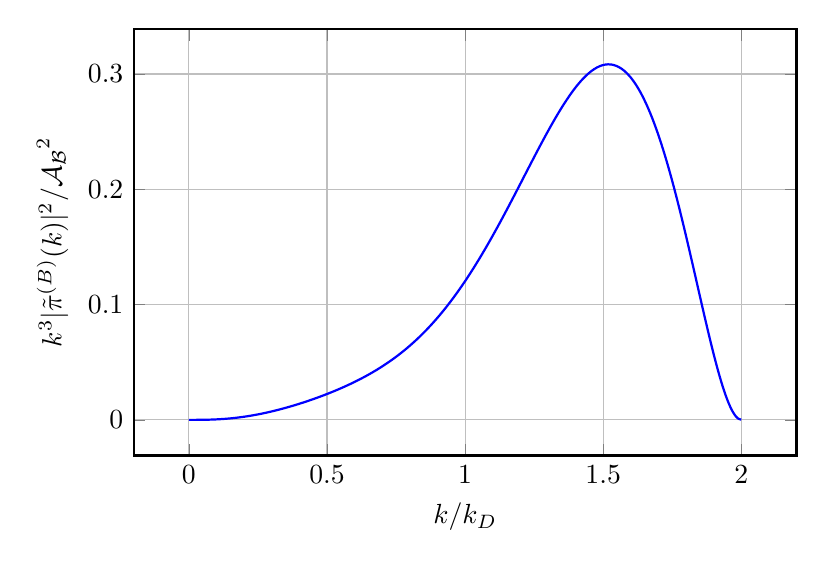
\begin{tikzpicture}
        \begin{axis}[
            width=10cm,
            height=7cm,
            xlabel={$k/k_D$},
            ylabel={$k^3 |\tilde{\pi}^{(B)}(k)|^2/ \mathcal{A_B}^2$ },
            domain=0:2,
            samples=200,
            grid=major,
            thick
        ]
        % The formula below is the normalized version:
        % y = k^3 * [8/15 - 7/6*k + 16/15*k^2 - 7/24*k^3 - 13/480*k^5 + 11/1920*k^7]
        \addplot[
            blue,
            smooth
        ] 
        {x^3 * (8/15 - 7/6*x + 16/15*x^2 - 7/24*x^3 - 13/480*x^5 + 11/1920*x^7)};
        \end{axis}
    \end{tikzpicture}
    \label{fig:stress_B}
    \caption{Plot of $k^3 |\tilde{\pi}^{(B)}(k)|^2$ for $n_B=2$ as a function of $k/k_D$. We can appreciate that the anisotropic stress has a peak right after $k_D$, to then vanish for $2k_D$.}
\end{figure}


Decomposing the gravitational wave in its two polarization and considering radiation domination $a \propto\tau$, we obtain the following differential equation for each polarization
$$
\tilde h_k''+\frac{2}{\tau}\tilde h_k'+\mathbf k^2\tilde h_k=\frac{6}{\tau^2}\frac{\tilde\pi^{(B)}}{\bar \rho_\gamma},
$$
where we used the Friedmann equation to obtain the time independent ratio $\tilde\pi^{(B)}/\bar\rho_\gamma$ (since numerator and denominator scale with the same power of $a(\tau)$). It is easy to check that the above equation, in the super Hubble horizon limit, has a logarithmically growing solution $h_k\propto\log (k\tau)$. This, at least in theory, would allow for an unbounded growth of the tensor modes. 